% !TEX root = main.tex

\section{実験2-1:画像処理実験}

\subsection{実験概要}
本実験では,手先に装着したRGB-Dカメラから取得した画像を処理し,
対象物体の検出および3次元位置情報の取得を実験する.
マニピュレータの卓上には,右角度の積み木(赤色,青色,黄色)および収納台が設置されており,
実験では積み木および各収納位置を対象に実験を行う.

\subsection{実験手順}
実験手順は以下の手順で行う.

\begin{enumerate}
  \item[(1)] 卓上に積み木を1個設置し,卓上の目盛りから各物体の$0^{\circ}xy$座標を直接計測し,記録する.
  \item[(2)] Pythonの開発環境Spyderを起動し,画像処理プログラムから空間フィルタリングをOFFにする.
  \item[(3)] 画像処理プログラムを実行後,マニピュレータの制御用ソフトウェアを用いてマニピュレータを手動操作し,画像に積み木が現れる位置まで手先を移動する.この際,手先の位置姿勢を記録する.
  \item[(4)] ヒストグラムを参考にしながら積み木のHSV色空間のしきい値(最大値,最小値)を設定し,記録する.また,スクリーンショット等を用いて,画像処理結果を記録する.
  \item[(5)] 得られた3次元位置情報を記録する.
  \item[(6)] 「平均化フィルタ」,「ガウシアンフィルタ」,「メディアンフィルタ」,「双方向フィルタ」において,それぞれ(1)~(5)を繰り返す.
  \item[(6)] 残りの積み木および収納位置を適所について,(1)~(6)を繰り返す.
  \item[(7)] 式(3.1)を用いて,座標変換を行い,物体の3次元位置をグローバル座標系で表現するエクセルファイルを作成し,計算する.
\end{enumerate}

\subsection{実験結果}
表6.1~表6.3に実験結果を示す.

\begin{table}[h]
  \centering
  \scriptsize % 文字サイズを小さくする
  \caption{積み木(赤)の結果}
  \begin{tabular}{|c|c|c|c|c|c|}
    \hline
                                                      & フィルタ無                                 & 平均フィルタ        & ガウシアンF         & メディアンF         & 双方向フィルタ      \\ \hline
    \hline
    実位置 ($x_{0}^{\circ}, y_{0}^{\circ}$) [mm]      & \multicolumn{5}{|c|}{ 488.5 ,-130.0  }                                                                                             \\ \hline
    手先位置 ($x_{e}^{\circ}, y_{e}^{\circ}, z$) [mm] & \multicolumn{5}{|c|}{401.1 , 0.0 , 418.2}                                                                                          \\ \hline
    手先姿勢 (R, P, Y) [deg]                          & \multicolumn{5}{|c|}{180, 0 , 0          }                                                                                         \\ \hline
    H(max, min)                                       & (3,0)                                      & (10,0)              & (10,0)              & (10,0)              & (10,0)              \\ \hline
    S(max, min)                                       & (255,60)                                   & (232,61)            & (255,60)            & (255,60)            & (255,60)            \\ \hline
    V(max, min)                                       & (255,0)                                    & (255,0)             & (255,0)             & (255,0)             & (255,95)            \\ \hline
    計測位置 ($x_{e}^{\circ}, y_{e}^{\circ}, z$) [mm] & (85.1 , 120.1 , 371)                       & (84.5,130.3,379.9)  & (85.0,128.6,377.9)  & (84.3,124.3,375.9)  & (85.0,126.9,375.9)  \\ \hline
    計測位置 ($x_{0}^{\circ}, y_{0}^{\circ}, z$) [mm] & (486.2,-120.1,47.2)                        & (485.6,-130.3,38.3) & (486.1,-128.6,40.3) & (485.4,-204.3,42.3) & (486.1,-126.9,42.3) \\ \hline
  \end{tabular}
\end{table}

\begin{table}[h]
  \centering
  \scriptsize % 文字サイズを小さくする
  \caption{積み木(青)の結果}
  \begin{tabular}{|c|c|c|c|c|c|}
    \hline
                                                      & フィルタ無                                & 平均フィルタ        & ガウシアンF         & メディアンF         & 双方向フィルタ      \\ \hline
    \hline
    実位置 ($x_{0}^{\circ}, y_{0}^{\circ}$) [mm]      & \multicolumn{5}{c|}{588.5 ,-130.0 }                                                                                               \\ \hline
    手先位置 ($x_{e}^{\circ}, y_{e}^{\circ}, z$) [mm] & \multicolumn{5}{c|}{401.1 , 0.0 , 418.2 }                                                                                         \\ \hline
    手先姿勢 (R, P, Y) [deg]                          & \multicolumn{5}{c|}{180, 0 , 0          }                                                                                         \\ \hline
    H(max, min)                                       & (160,140)                                 & (160,140)           & (160,140)           & (160,140)           & (160,140)           \\ \hline
    S(max, min)                                       & (255,60)                                  & (255,60)            & (255,60)            & (255,60)            & (255,60)            \\ \hline
    V(max, min)                                       & (255,0)                                   & (255,0)             & (255,0)             & (255,0)             & (255,0)             \\ \hline
    計測位置 ($x_{e}^{\circ}, y_{e}^{\circ}, z$) [mm] & (181.6,128.1,374.9)                       & (182.7,131.5,377.9) & (182.1,129.7,375.9) & (182.4,129.0,375.9) & (180.7,127.4,375.9) \\ \hline
    計測位置 ($x_{0}^{\circ}, y_{0}^{\circ}, z$) [mm] & (582.7,-128.1,43.3)                       & (583.1,-131.5,40.3) & (583.2,-129.7,42.3) & (583.5,-129.0,42.3) & (581.8,-127.4,42.3) \\ \hline
  \end{tabular}
\end{table}

\begin{table}[h]
  \centering
  \scriptsize % 文字サイズを小さくする
  \caption{積み木(黄)の結果}
  \begin{tabular}{|c|c|c|c|c|c|}
    \hline
                                                      & フィルタ無                                 & 平均フィルタ        & ガウシアンF         & メディアンF         & 双方向フィルタ      \\ \hline
    \hline
    実位置 ($x_{0}^{\circ}, y_{0}^{\circ}$) [mm]      & \multicolumn{5}{c|}{388.5 ,-130.0  }                                                                                               \\ \hline
    手先位置 ($x_{e}^{\circ}, y_{e}^{\circ}, z$) [mm] & \multicolumn{5}{c|}{401.1 , 0.0 , 418.2  }                                                                                         \\ \hline
    手先姿勢 (R, P, Y) [deg]                          & \multicolumn{5}{c|}{180, 0 , 0 }                                                                                                   \\ \hline
    H(max, min)                                       & (50,30)                                    & (50,30)             & (50,30)             & (50,30)             & (50,30)             \\ \hline 
    S(max, min)                                       & (255,60)                                   & (255,60)            & (255,60)            & (255,60)            & (255,60)            \\ \hline
    V(max, min)                                       & (255,0)                                    & (255,0)             & (255,0)             & (255,0)             & (255,0)             \\ \hline
    計測位置 ($x_{e}^{\circ}, y_{e}^{\circ}, z$) [mm] & (-12.3,119.9,365.9)                        & (-15.0,124.7,370.9) & (-13.0,121.9,366.9) & (-13.0,117.2,365.9) & (-13.0,121.2,365.9) \\ \hline
    計測位置 ($x_{0}^{\circ}, y_{0}^{\circ}, z$) [mm] & (338.8,-119.9,52.3)                        & (386.1,-124.7,47.3) & (388.1,-121.9,51.3) & (388.1,-117.2,52.3) & (-13.0,121.2,365.9) \\ \hline
  \end{tabular}
\end{table}
\newpage

次に,図6.1に各フィルタの誤差率のグラフを示す.

\begin{figure}[H]
  \centering
  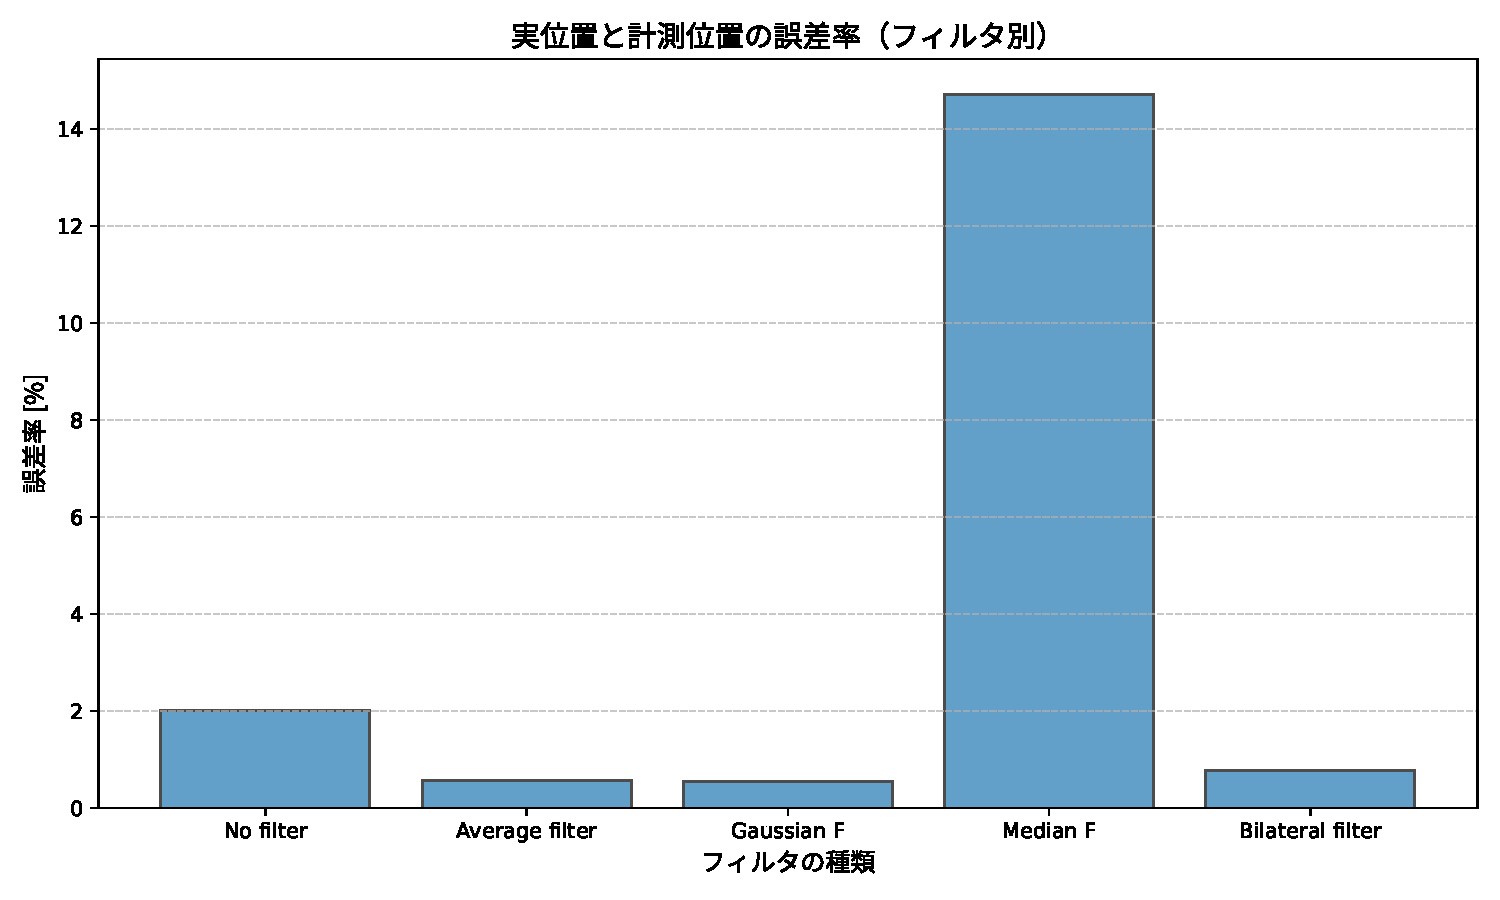
\includegraphics[scale=0.7]{sozai/gurafu.pdf}
  \caption{各フィルタの誤差率のグラフ}
\end{figure}

次に,図6.5から図6.6に赤ブロックのフィルタ後の画像を示す.

\begin{figure}[H]
  \centering
  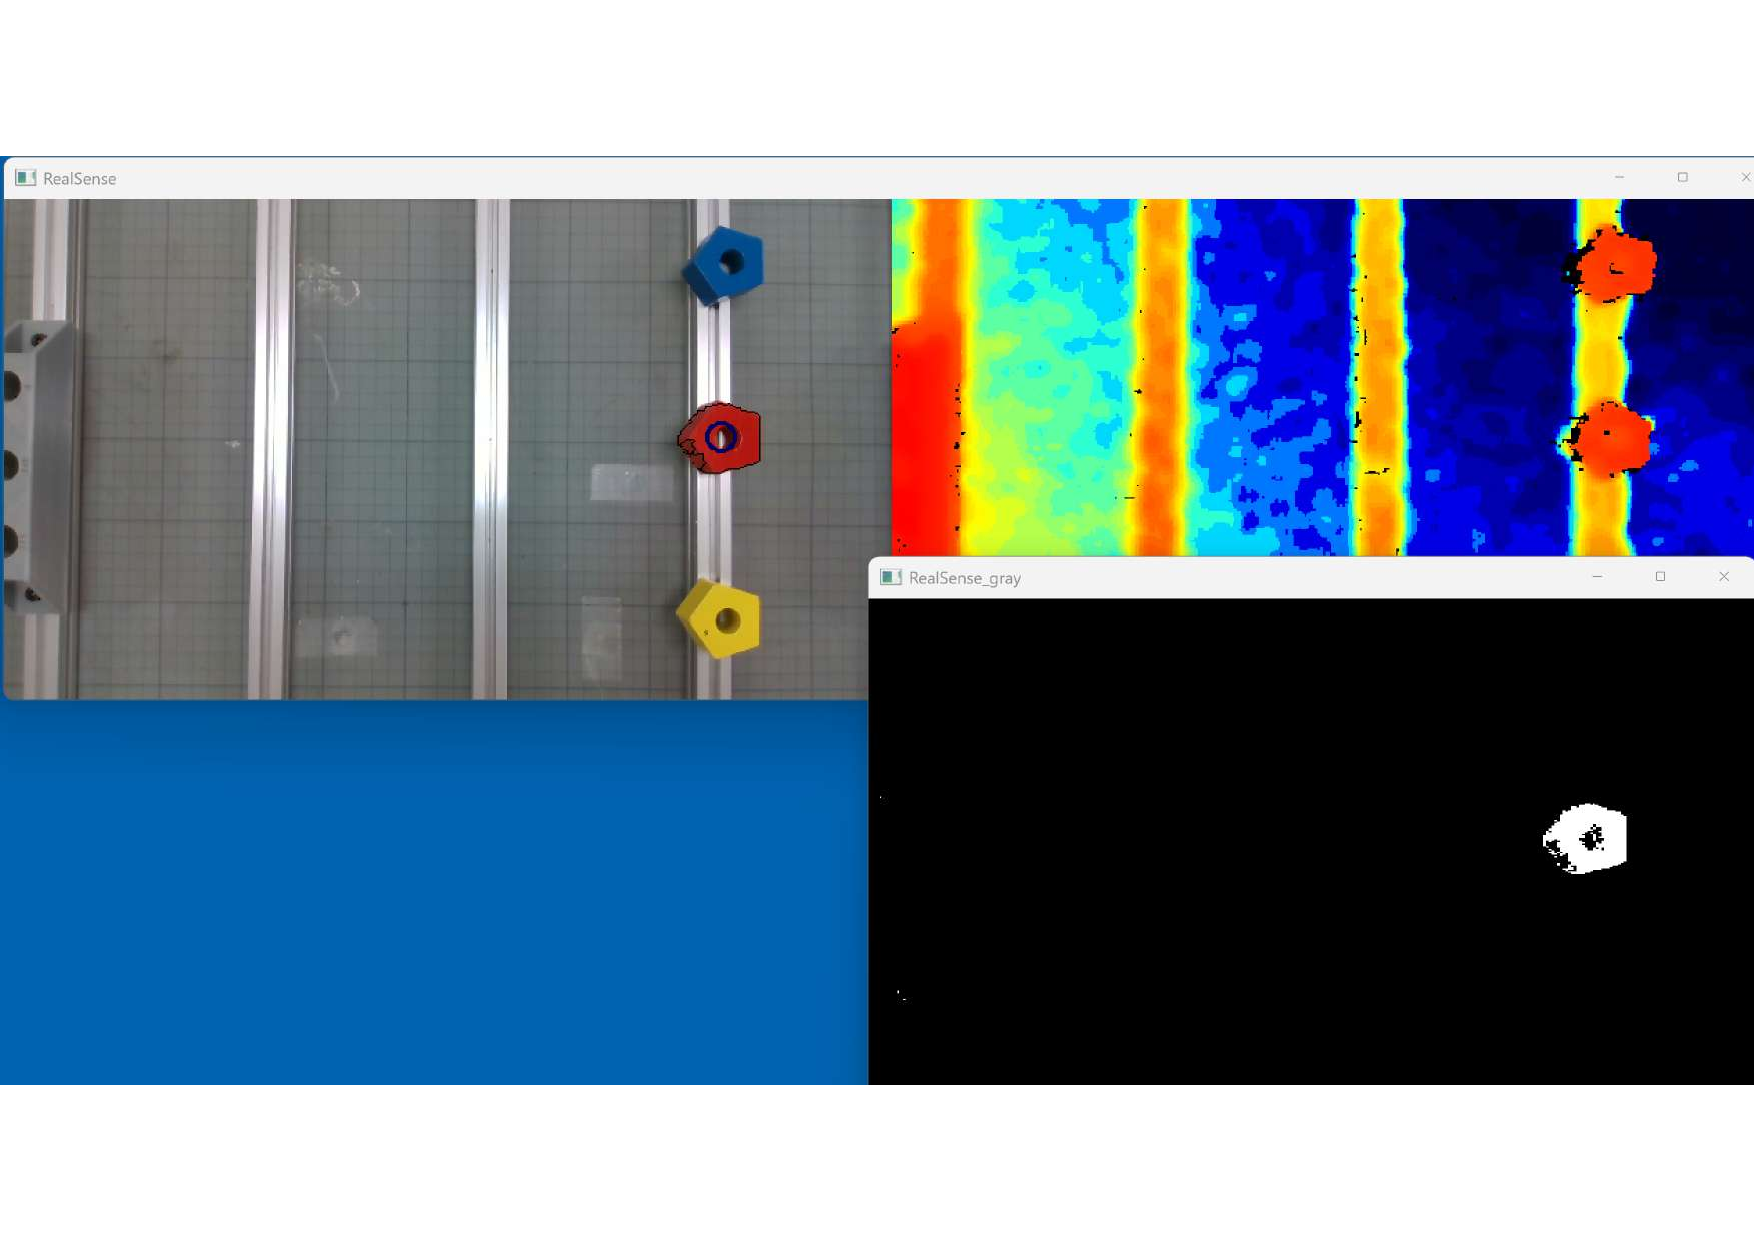
\includegraphics[scale=0.5]{sozai/a.pdf}
  \caption{赤フィルタなし}
\end{figure}

\begin{figure}[H]
  \centering
  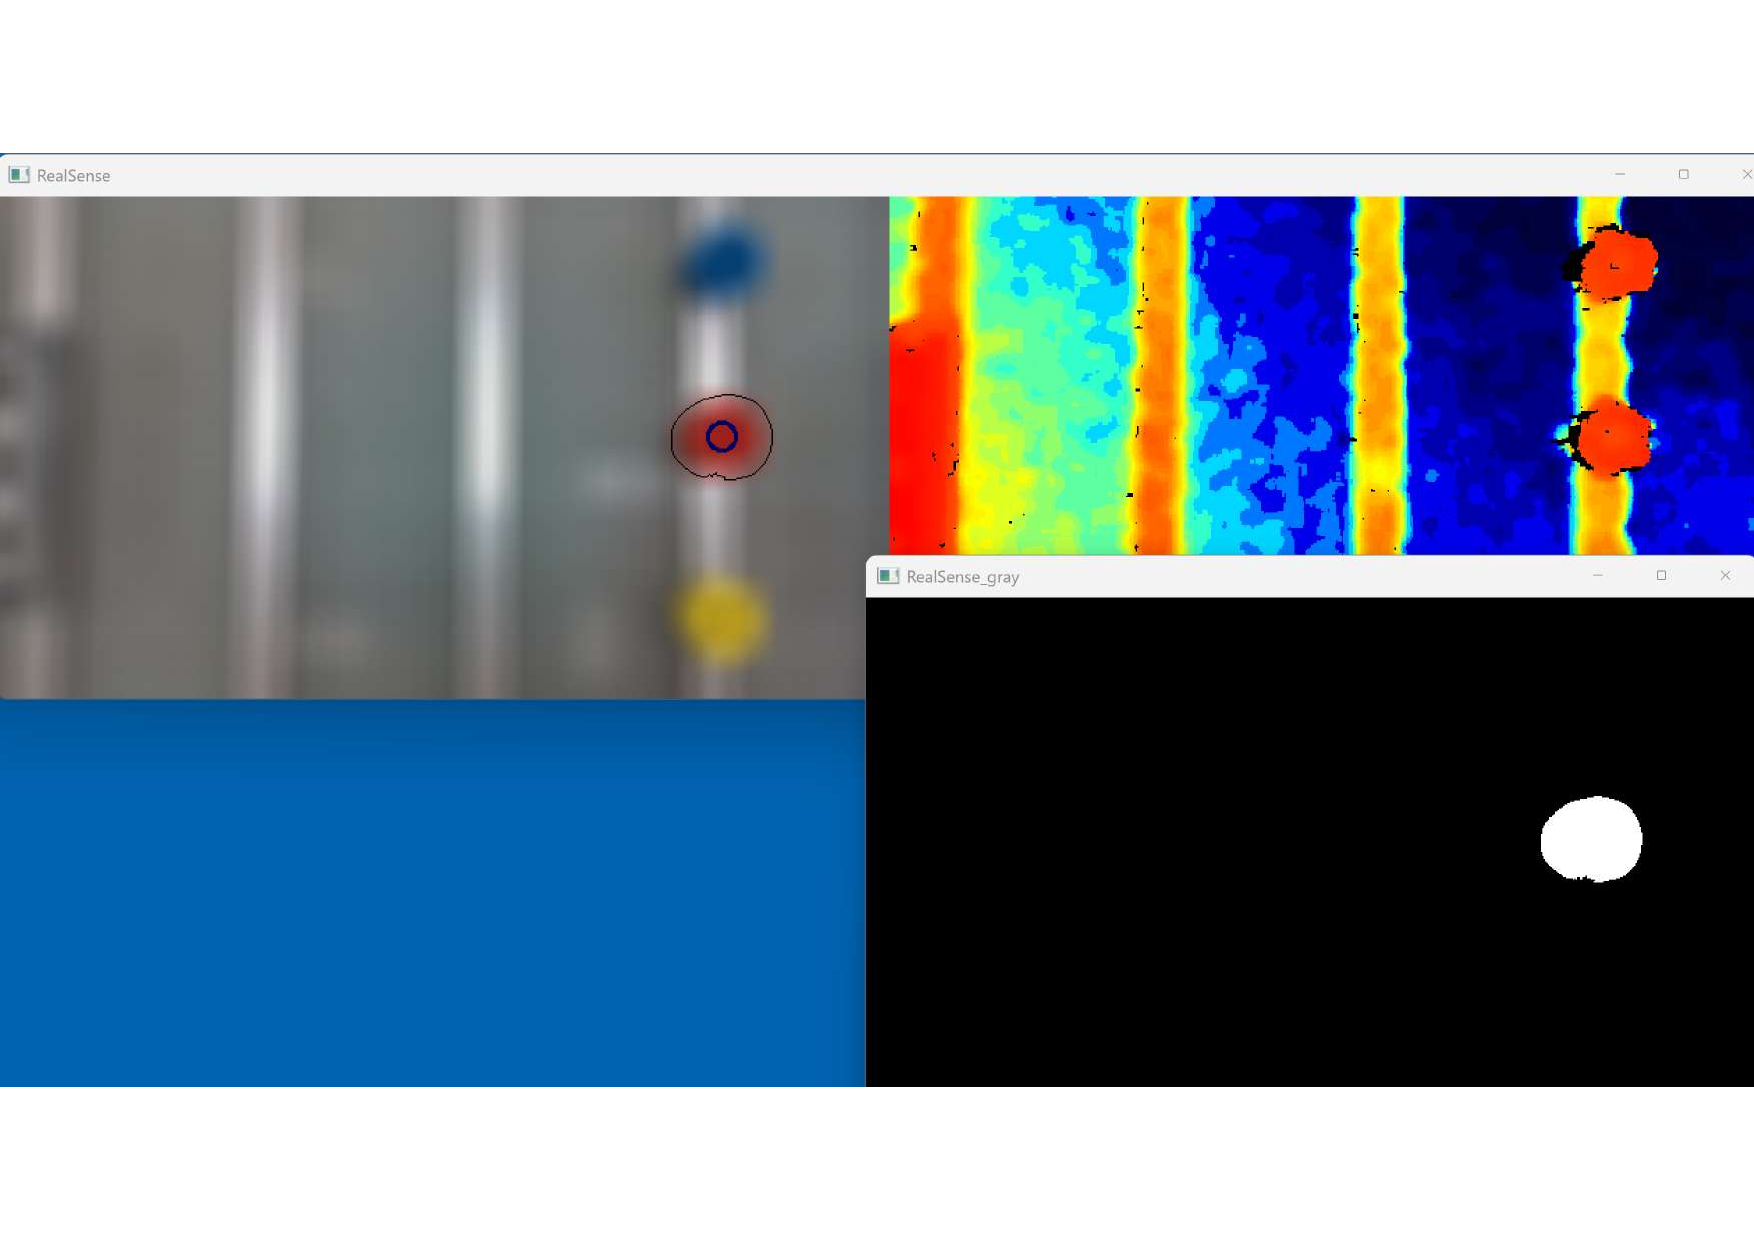
\includegraphics[scale=0.5]{sozai/b.pdf}
  \caption{赤平均フィルタ}
\end{figure}

\begin{figure}[H]
  \centering
  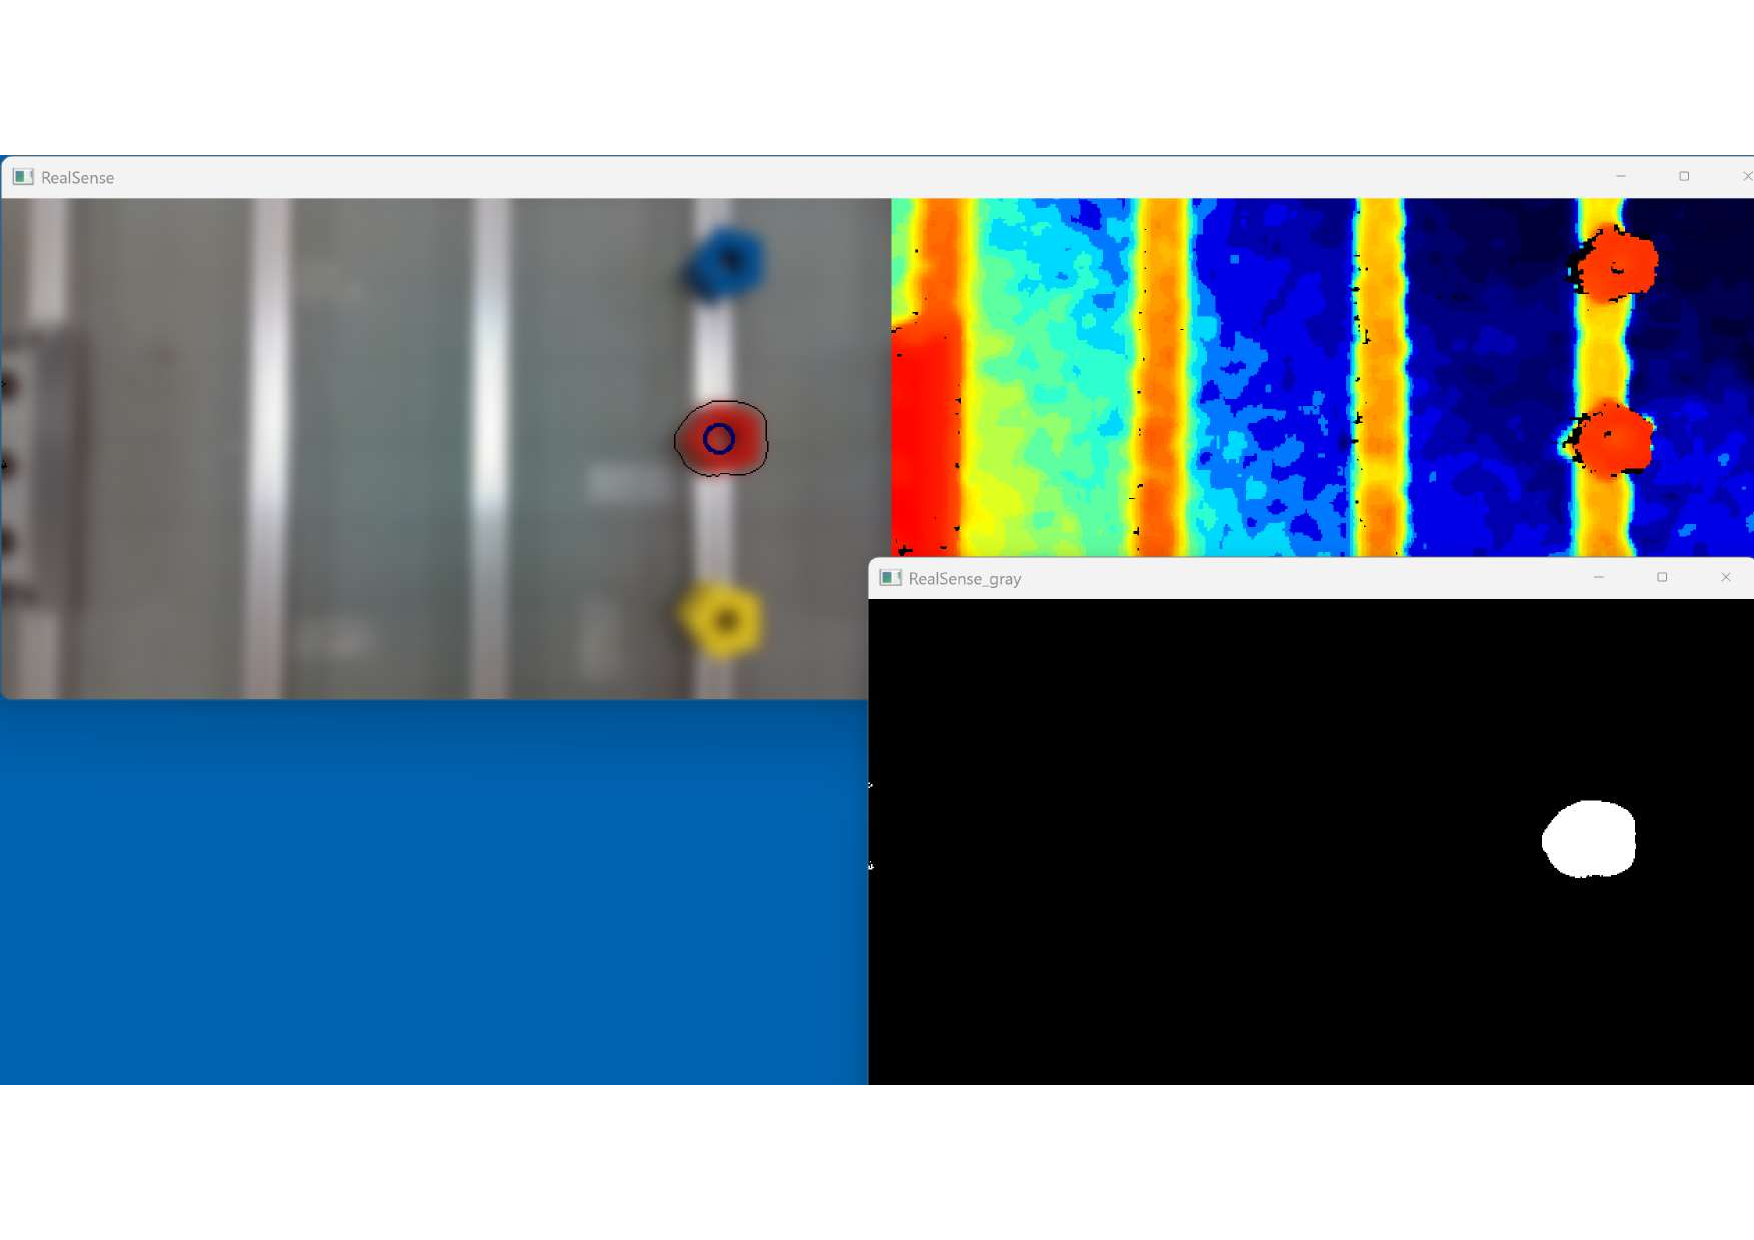
\includegraphics[scale=0.5]{sozai/c.pdf}
  \caption{赤ガウシアン}
\end{figure}

\begin{figure}[H]
  \centering
  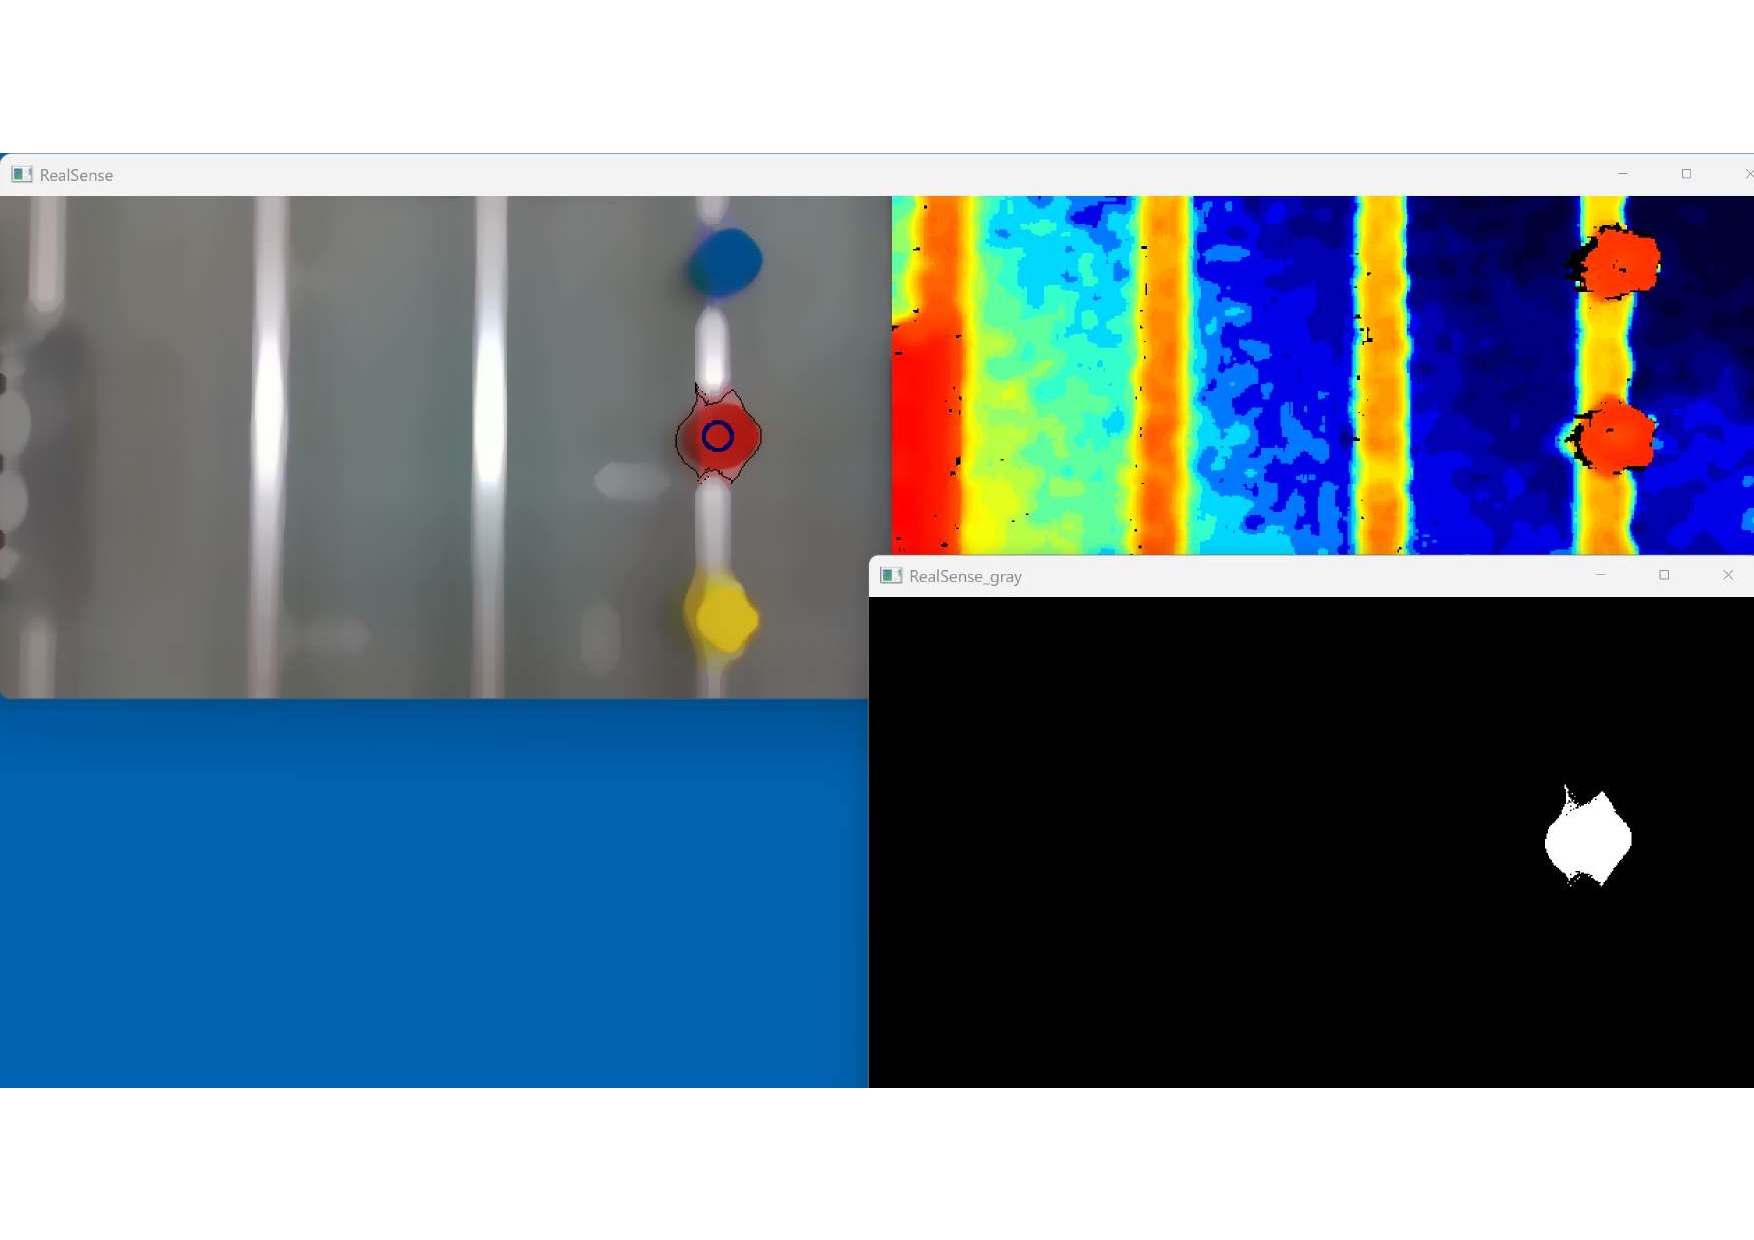
\includegraphics[scale=0.5]{sozai/d.pdf}
  \caption{赤メディアン}
\end{figure}

\begin{figure}[H]
  \centering
  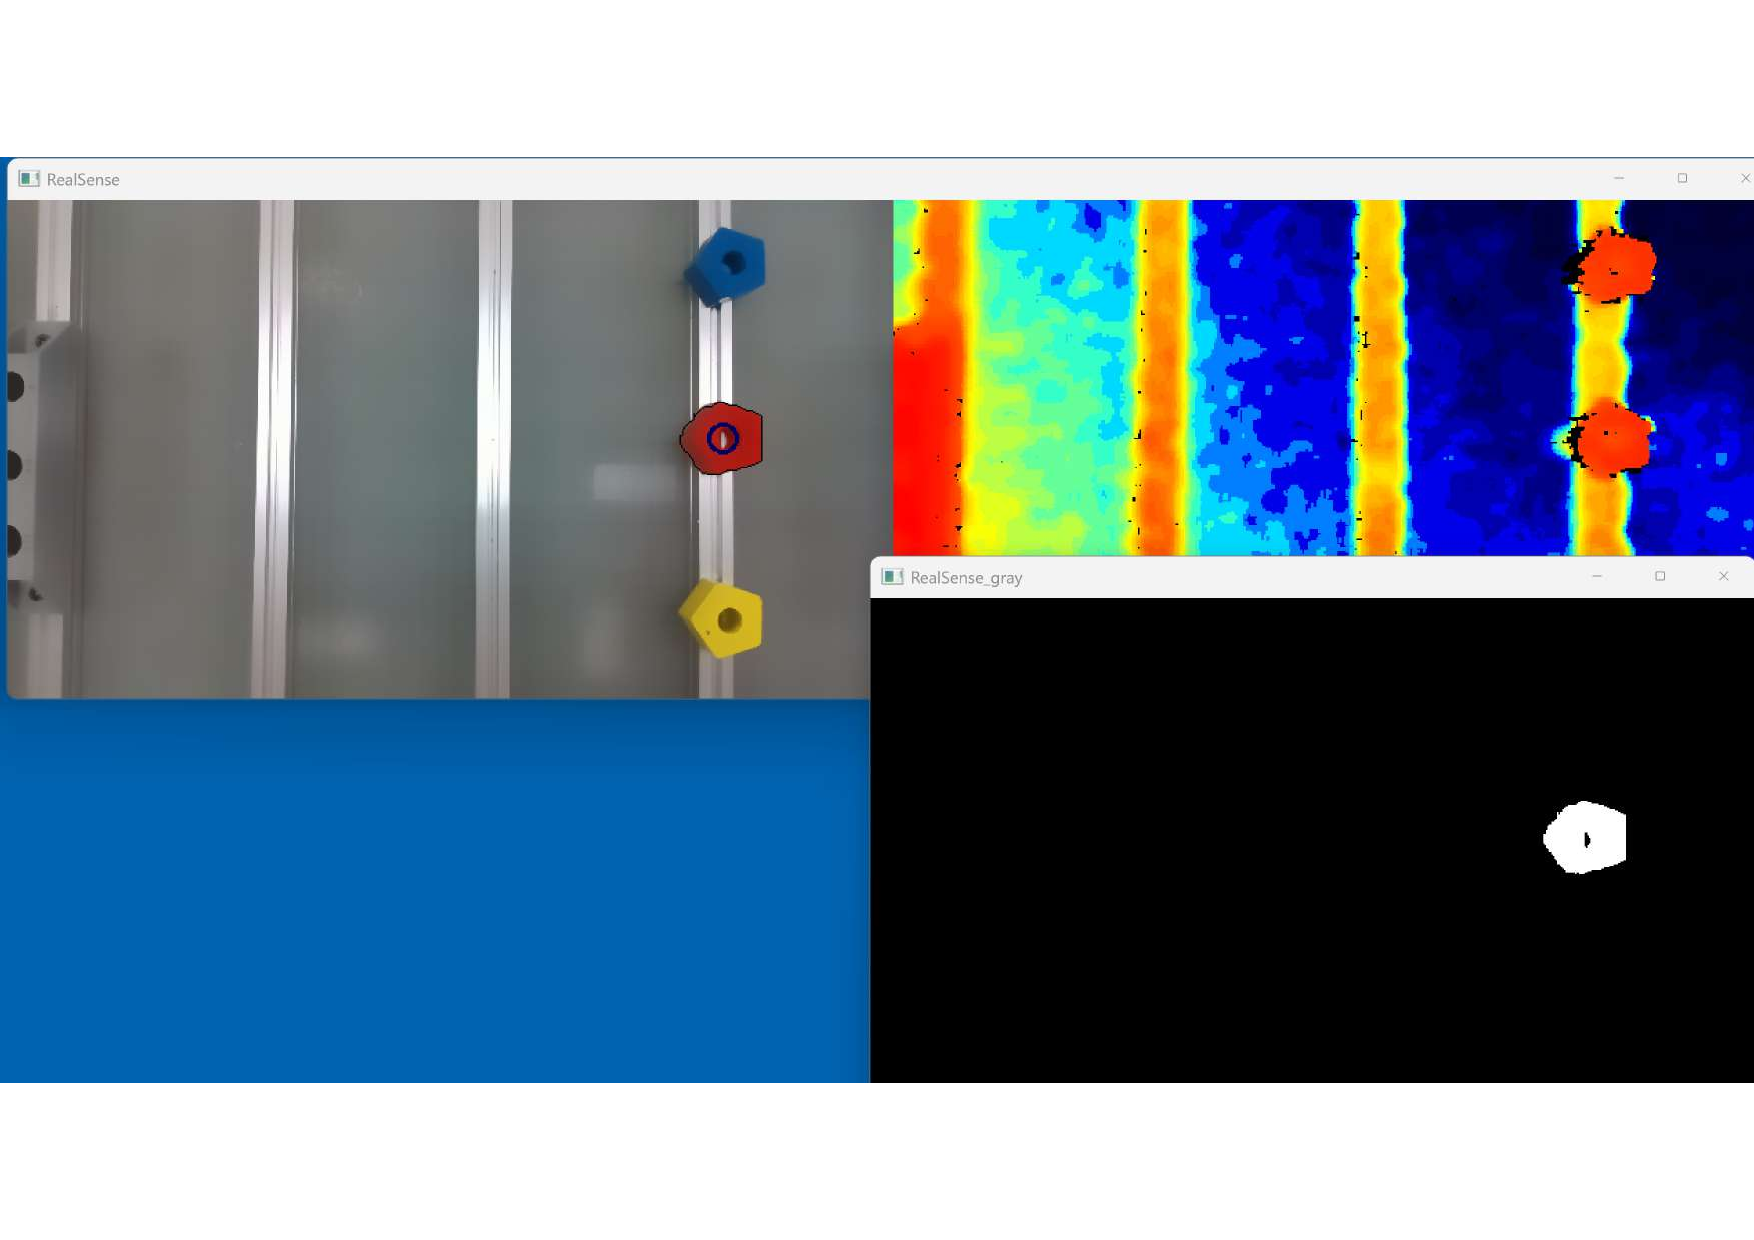
\includegraphics[scale=0.5]{sozai/e.pdf}
  \caption{赤双方向}
\end{figure}



\subsection{考察}
本実験において,実位置と計測結果の誤差が生じた要因を以下に考察する.

フィルタリング処理の種類により,画像の平滑化やノイズ除去の効果が異なるため,
計測位置に差異が生じたと考えられる.たとえば,メディアンフィルタはランダムノイズの除去に優れる一方で,
エッジ部分を損なう可能性がある.一方,ガウシアンフィルタや双方向フィルタは全体的な平滑化に優れるが,
細かなエッジ情報を維持しにくい場合がある.これらの特性が,計測位置の差異を引き起こした要因と考えられる.

他には,カメラの位置によってブロックの見え方や影響が変わり,二値化画像の生成に影響を与えた可能性がある.
例えば,カメラがブロックに対して角度を持って設置されている場合,
画像上の歪みが発生し,計測位置に誤差が生じたと推測される.
また,光源の位置や反射が二値化結果に影響を及ぼし,HSV空間での閾値設定にも影響を与えた可能性がある.

空間フィルタリングは,二値化処理の前段階でノイズを除去し,画像のエッジを強調する役割を持つ.
フィルタ処理を行わない場合,ノイズがそのまま画像に残り,
二値化処理の際にエッジが不正確になる可能性が高い. 平均フィルタは全体的な平滑化効果があるが,
エッジ部分も平滑化されるため,ブロックの輪郭がぼやける可能性がある.ガウシアンフィルタは画像全体を滑らかにするが,
エッジのぼやけは平均フィルタより少ない.ただし,ノイズの除去が不完全な場合がある.
メディアンフィルタはランダムノイズの除去に優れるため,
二値化画像のエッジが比較的はっきりする.ただし,エッジ付近で異常値を検出する可能性がある.
双方向フィルタは,ノイズ除去とエッジ保持のバランスが良い.
本実験では平均フィルタを用いた例が1番誤差が少なかったが,これはぼやかすことにより,
より測定した中心がより中心に近づいたからだと考えられる.


\section{実験2-2:3次元位置計測と物体の把持収納実験}

\subsection{実験概要}
本実験では,手先に装着したRGB-Dカメラから把持物体および収納位置の3次元位置情報を取得し,
物体の把持および収納する実験を行う.図7.1に実験環境の模式図を示す.マニピュレータの卓上には,
把持する五角形の積み木(赤色,青色,黄色)と収納位置用の積み木(黄,青,緑)が置かれている.
マニピュレータは五角形形の積み木を検出・把持して収納位置に配置する動作を行う.

\subsection{実験手順}
実験手順は以下の手順で行う.

\begin{enumerate}
  \item[(1)] 卓上に積み木を3個,収納台座をすべて無造作に配置する.
  \item[(2)] Pythonの開発環境Spyderを起動し,実験3において最も優れた結果となった空間フィルタリングを選択する.
  \item[(3)] 画像処理プログラムを実行後,マニピュレータの制御用ソフトウェアを用いてマニピュレータを手動操作し,画像に各物体が現れる位置まで手先を移動する.この際,手先の位置姿勢を記録する.
  \item[(4)] 実験3で記録したHSV色空間のしきい値を設定し,各物体の検出を行う.また,実験3で作成したエクセルを用いて,各物体の3次元位置をグローバル座標系で表現する.
  \item[(5)] マニピュレータの制御用ソフトウェアを用いて,手先位置の数値指定によるオンラインティーチングを行う.動作は,赤積み木の把持収納,青積み木の把持収納,黄積み木の把持収納をすべて連続で行う.ただし,手先の姿勢$(R, P, Y) = (180, 0, 0)$ [deg]とし,手先の$0^{\circ}$位置を80[mm](把持時),110[mm](収納時)とすること.また,動作の様子を動画撮影する.
\end{enumerate}

\subsection{実験結果}
表7.1に実験結果を示す.また,図7.2にマニピュレータが積み木を把持・収納する様子を示す.

\begin{table}[h]
  \centering
  \scriptsize % 文字サイズを小さくする
  \caption{物体の位置}
  \begin{tabular}{|c|c|c|c|c|c|c|}
    \hline
                                             & 赤積木                                     & 青積木                & 黄積木                & 赤収納              & 青収納              & 黄収納              \\ \hline
    \hline
    ($x_{0}^{\circ}, y_{0}^{\circ}, z$) [mm] & \multicolumn{6}{|c|}{401.1 , 0.0 , 418.2 }                                                                                                                   \\ \hline
    (R, P, Y) [deg]                          & \multicolumn{6}{|c|}{180,0,0             }                                                                                                                   \\ \hline
    ($x_{e}^{\circ}, y_{e}^{\circ}, z$) [mm] & 84.5,130.3,37                              & 182.7 , 131.5 , 377.9 & -150, 124.7 , 370.9   & (177.7,126.6,375.9) & (88.7,-129.5,372.9) & (-5.7,-128.8,365.9) \\ \hline
    ($x_{0}^{\circ}, y_{0}^{\circ}, z$) [mm] & 482.6 , -130.3 ,38.3                       & 583.1 , -131.5 , 41.3 & 386.1 , -124.7 , 47.3 & (578.8,-126.6,42.3) & (489.9,129.545.3)   & (395.4,128.852.3)   \\ \hline
    成功                                     & 成功                                       & 成功                  & 成功                  & 成功                & 成功                & 失敗                \\ \hline 
    
  \end{tabular}
\end{table}

\begin{figure}[H]
  \centering
  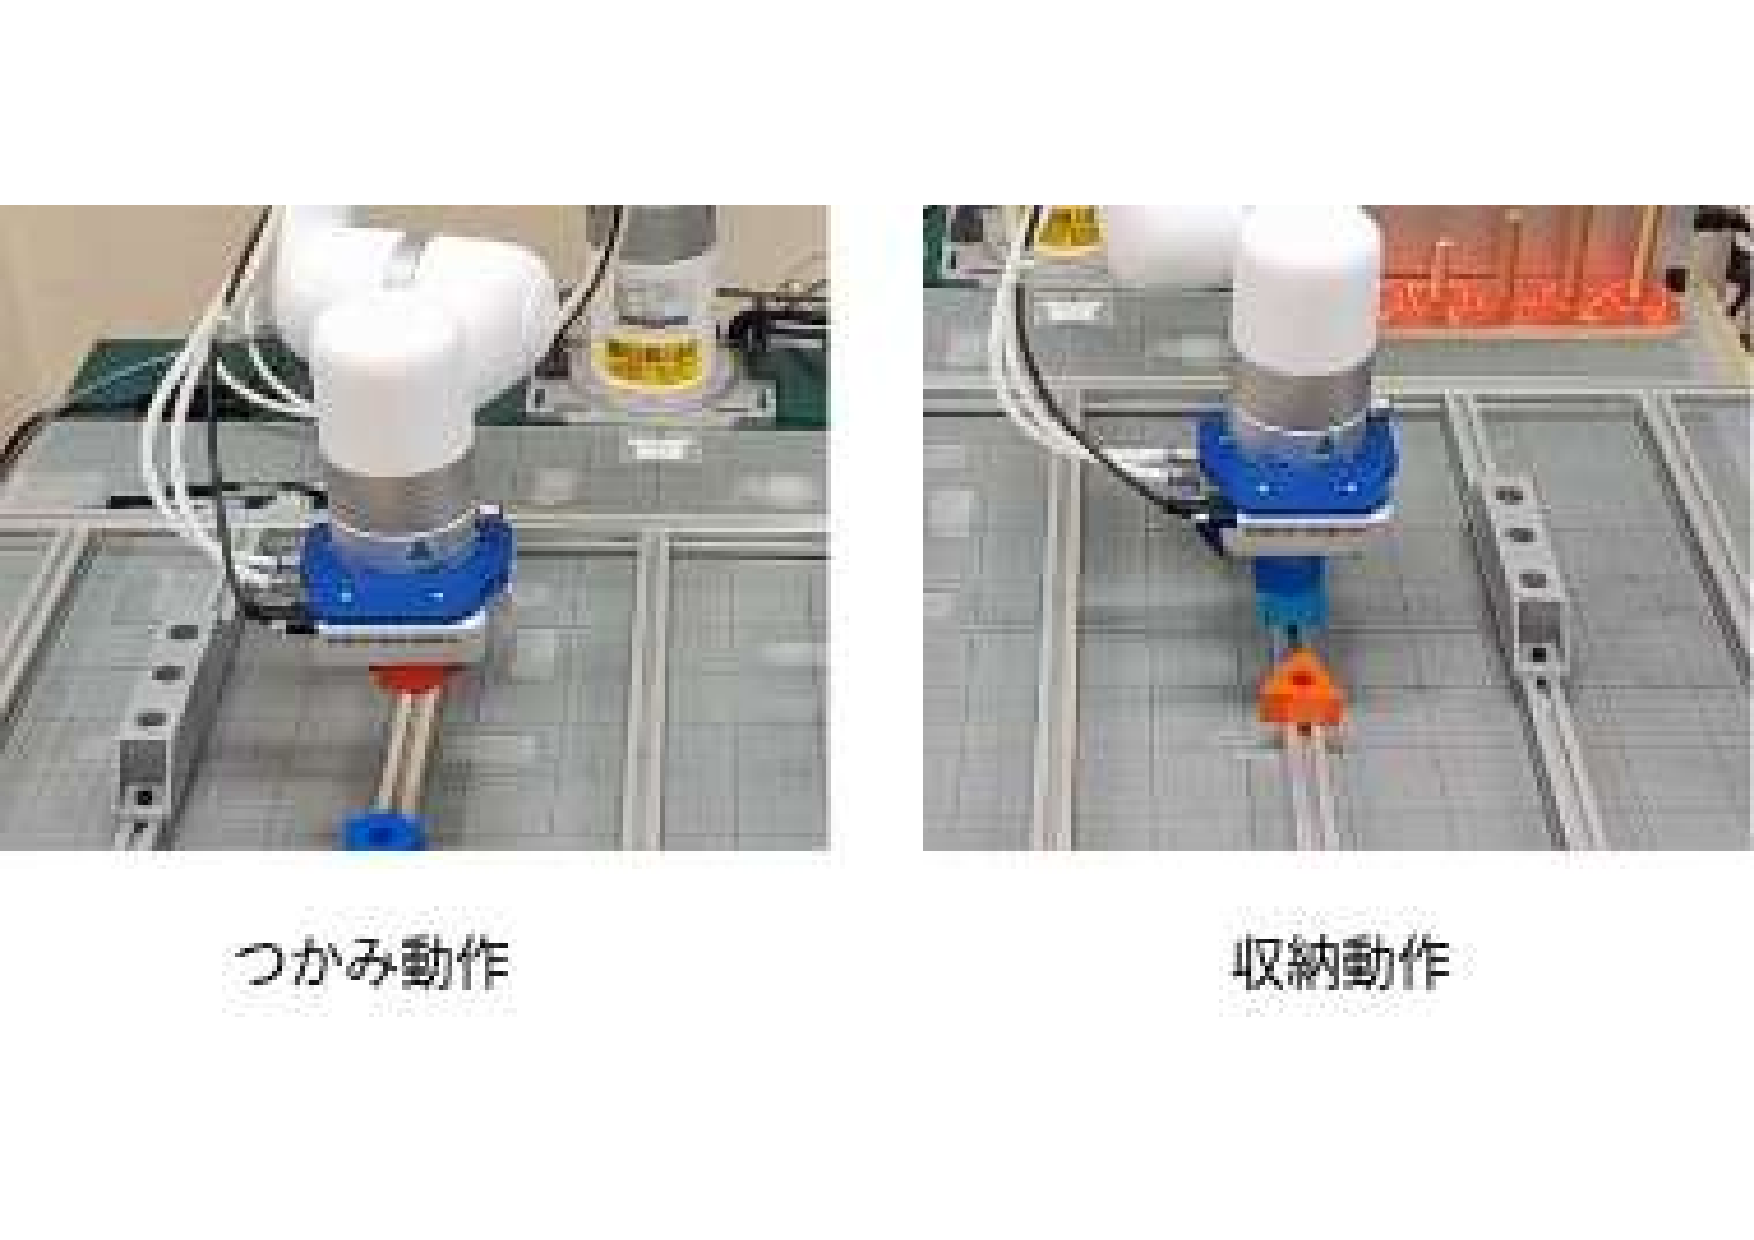
\includegraphics[scale=0.5]{sozai/8.pdf}
  \caption{保持する様子}
\end{figure}

平均フィルタで得られた位置をもとにロボットアームを動作させた.
少し掴むものからずれていても,アームの手を閉じると掴むことができていた.

\subsection{考察}
次に,考察を行う.
本実験で使用したロボットアームのグリッパは,把持時に「手」を閉じる動作を通じて対象物を固定する構造を
持っている.この構造により,対象物の位置に多少の誤差が生じた場合でも,把持を成功させることが可能である.
特に,赤積木と青積木は手先位置が完全に一致しない場合でも,グリッパが自動的に物体を挟む動作により,
成功率を高める結果となった.

%%%%%%%%%%%%%%%%%%%%%%%%%%%%%%%%%%%%%%%%%%%%%%%%%%%%%%%%%%%%%%%
\section{課題}

\subsection{逆運動学の導出}
\subsubsection{式(2.6)の導出}

手先位置$\begin{bmatrix} x_0 \\ y_0 \\ z_0 \end{bmatrix}$がグローバル座標系で与えられているとき,座標系$\Sigma$における手先位置は以下のように変換される:

\[
  \begin{bmatrix} x \\ y \\ z \end{bmatrix} = \begin{bmatrix} x_0 \\ y_0 \\ z_0 - l_1 \end{bmatrix} \tag{2.4}
\]

ここで,$xy$平面に注目すると,関節角度$\theta_1$は,$x$軸と手先位置$\begin{bmatrix} x \\ y \end{bmatrix}$がなす角度として定義される.$\tan^{-1}(y/x)$では範囲が$[-\pi/2, \pi/2]$に制限される場合があるため,$\text{atan2}$を用いて次の式を得る:

\[
  \theta_1 = \text{atan2}(y, x) \tag{2.6}
\]

\subsubsection{式(2.12)の導出}

$xy$平面における原点から手先位置への距離(射影距離)を計算する.これはピタゴラスの定理を適用することで以下のように求められる:

\[
  |x'| = \sqrt{x^2 + y^2} \tag{2.7}
\]

正負の符号を考慮して絶対値を外すと,

\[
  x' = \pm \sqrt{x^2 + y^2} \tag{2.8}
\]

次に,$x'z'$平面に注目する.$l_2$, $l_3$, $x'$, $z$からなる三角形を考えると,余弦定理を適用できる.余弦定理の一般形は次の通り:

\[
  c^2 = a^2 + b^2 - 2ab \cos \theta \tag{2.9}
\]

ここで,
\[
  a = l_2 \quad \text{(第2関節から第3関節までのリンク長)}
\]
\[
  b = l_3 \quad \text{(第3関節から手先位置までのリンク長)}
\]
\[
  c = \sqrt{x'^2 + z^2} \quad \text{($x'z'$平面上の手先位置から原点までの距離)}
\]
\[
  \theta = \varphi_2 - \theta_3 \text{(角度)}
\]

を代入する.
このとき,次の式が成立する:

\[
  x'^2 + z^2 = l_2^2 + l_3^2 - 2l_2 l_3 \cos (\varphi_2 - \theta_3)
\]

これを変形すると,

\[
  \cos(\varphi_2 - \theta_3) = \frac{l_2^2 + l_3^2 - x'^2 - z^2}{2 l_2 l_3} \tag{2.10}
\]

さらに,三角関数の関係式,

\[
  \sin^2 \theta + \cos^2 \theta = 1
\]

を用いて,$\sin(\varphi_2 - \theta_3)$を次のように表せる:

\[
  \sin(\varphi_2 - \theta_3) = \pm \sqrt{1 - \cos^2 (\varphi_2 - \theta_3)} \tag{2.11}
\]

ここで,$\cos(\varphi_2 - \theta_3)$と$\sin(\varphi_2 - \theta_3)$が求まったので,$\text{atan2}$を適用して$\theta_3$を計算する:

\[
  \theta_3 = \varphi_2 - \text{atan2} \{ \sin(\varphi_2 - \theta_3), \cos(\varphi_2 - \theta_3) \} \tag{2.12}
\]

\subsubsection{式(2.13)~式(2.14)の導出}

関節角度$\theta_2$を求めるために,順運動学の式を逆に利用する.リンク2とリンク3の動作を順運動学で記述すると,$x'$軸方向と$z$軸方向の動きは次のように表される:

\[
  x' = K_c \cos(\varphi_1 - \theta_2) - K_s \sin(\varphi_1 - \theta_2) \tag{2.13a}
\]

\[
  z = K_s \cos(\varphi_1 - \theta_2) + K_c \sin(\varphi_1 - \theta_2) \tag{2.13b}
\]

ここで,以下の定義を用いる:

\[
  K_c = l_2 + l_3 \cos \theta_3, \quad K_s = l_3 \sin \theta_3
\]

これらを用いて,$\tan(\varphi_1 - \theta_2)$を計算するために正弦と余弦の比を取る.


式(2.13a)を$\cos(\varphi_1 - \theta_2)$で整理する:

\[
  x' = K_c \cos(\varphi_1 - \theta_2) - K_s \sin(\varphi_1 - \theta_2)
\]

\[
  \Rightarrow x' + K_s \sin(\varphi_1 - \theta_2) = K_c \cos(\varphi_1 - \theta_2)
\]

\[
  \Rightarrow \cos(\varphi_1 - \theta_2) = \frac{x' + K_s \sin(\varphi_1 - \theta_2)}{K_c}
\]

次に,式(2.13b)を$\sin(\varphi_1 - \theta_2)$で整理する:

\[
  z = K_s \cos(\varphi_1 - \theta_2) + K_c \sin(\varphi_1 - \theta_2)
\]

\[
  \Rightarrow z - K_s \cos(\varphi_1 - \theta_2) = K_c \sin(\varphi_1 - \theta_2)
\]

\[
  \Rightarrow \sin(\varphi_1 - \theta_2) = \frac{z - K_s \cos(\varphi_1 - \theta_2)}{K_c}
\]

これらを用いて,正弦と余弦の比を計算する:

\[
  \tan(\varphi_1 - \theta_2) = \frac{\sin(\varphi_1 - \theta_2)}{\cos(\varphi_1 - \theta_2)}
\]

$\sin(\varphi_1 - \theta_2)$と$\cos(\varphi_1 - \theta_2)$をそれぞれ代入する:

\[
  \tan(\varphi_1 - \theta_2) = \frac{\frac{z - K_s \cos(\varphi_1 - \theta_2)}{K_c}}{\frac{x' + K_s \sin(\varphi_1 - \theta_2)}{K_c}}
\]

分母と分子を整理する:

\[
  \tan(\varphi_1 - \theta_2) = \frac{z - K_s \cos(\varphi_1 - \theta_2)}{x' + K_s \sin(\varphi_1 - \theta_2)}
\]

ここで,$\sin(\varphi_1 - \theta_2)$と$\cos(\varphi_1 - \theta_2)$を具体的に代入する代わりに,上記を簡略化して次の形で整理する:

\[
  \tan(\varphi_1 - \theta_2) = \frac{K_s x' + K_c z}{K_c x' - K_s z}
\]

$\tan(\varphi_1 - \theta_2)$を$\text{atan2}$を用いて直接表現すると:

\[
  \theta_2 = \varphi_1 - \text{atan2}\left( K_s x' + K_c z, K_c x' - K_s z \right) \tag{2.14}
\]

\subsection{回転行列とオイラー角の変換式}
課題:式(2.17)~式(2.20)を導出せよ.手書き可.ただし,枠や枠内の文章は報告書に記載不要とする.
参考文献は報告書最後の参考文献の欄に記載すること.

固定角を用いて姿勢を表現する際,回転行列$\mathbf{R}$は$x$軸(roll, $\phi$),$y$軸(pitch, $\theta$),$z$軸(yaw, $\psi$)の回転を順に適用して得られる.各軸周りの回転行列を以下のように定義する:

$z$軸周りの回転(yaw, $\psi$):
\[
  R_z = \begin{bmatrix} 
    \cos \psi & -\sin \psi & 0  \\ 
    \sin \psi & \cos \psi  & 0  \\ 
    0         & 0          & 1 
  \end{bmatrix}
\]

$y$軸周りの回転(pitch, $\theta$):
\[
  R_y = \begin{bmatrix} 
    \cos \theta  & 0 & \sin \theta  \\ 
    0            & 1 & 0            \\ 
    -\sin \theta & 0 & \cos \theta 
  \end{bmatrix}
\]

$x$軸周りの回転(roll, $\phi$):
\[
  R_x = \begin{bmatrix} 
    1 & 0         & 0          \\ 
    0 & \cos \phi & -\sin \phi \\ 
    0 & \sin \phi & \cos \phi 
  \end{bmatrix}
\]

これらを順に掛け合わせることで,全体の回転行列$\mathbf{R}$が得られる:

\[
  ^0\mathbf{R} = R_z R_y R_x
\]

まず,$R_z$と$R_y$を掛け合わせる:

\[
  R_z R_y = \begin{bmatrix} 
    \cos \psi & -\sin \psi & 0  \\ 
    \sin \psi & \cos \psi  & 0  \\ 
    0         & 0          & 1 
  \end{bmatrix}
  \begin{bmatrix} 
    \cos \theta  & 0 & \sin \theta  \\ 
    0            & 1 & 0            \\ 
    -\sin \theta & 0 & \cos \theta 
  \end{bmatrix}
\]

行列の積を成分ごとに計算する:

$(1,1)$成分:$\cos \psi \cdot \cos \theta + (-\sin \psi) \cdot 0 + 0 \cdot (-\sin \theta) = \cos \psi \cos \theta$

$(1,2)$成分:$\cos \psi \cdot 0 + (-\sin \psi) \cdot 1 + 0 \cdot 0 = -\sin \psi$

$(1,3)$成分:$\cos \psi \cdot \sin \theta + (-\sin \psi) \cdot 0 + 0 \cdot \cos \theta = \cos \psi \sin \theta$

以下同様に計算を進めると:

\[
  R_z R_y = \begin{bmatrix} 
    \cos \psi \cos \theta & -\sin \psi & \cos \psi \sin \theta \\ 
    \sin \psi \cos \theta & \cos \psi  & \sin \psi \sin \theta \\ 
    -\sin \theta          & 0          & \cos \theta 
  \end{bmatrix}
\]

次に,この結果に$R_x$を掛け合わせる:

\[
  ^0\mathbf{R} = \begin{bmatrix} 
    \cos \psi \cos \theta & -\sin \psi & \cos \psi \sin \theta \\ 
    \sin \psi \cos \theta & \cos \psi  & \sin \psi \sin \theta \\ 
    -\sin \theta          & 0          & \cos \theta 
  \end{bmatrix}
  \begin{bmatrix} 
    1 & 0         & 0          \\ 
    0 & \cos \phi & -\sin \phi \\ 
    0 & \sin \phi & \cos \phi 
  \end{bmatrix}
\]

行列積を成分ごとに計算すると:

$(1,1)$成分:$\cos \psi \cos \theta \cdot 1 + (-\sin \psi) \cdot 0 + \cos \psi \sin \theta \cdot 0 = \cos \psi \cos \theta$

$(1,2)$成分:$\cos \psi \cos \theta \cdot 0 + (-\sin \psi) \cdot \cos \phi + \cos \psi \sin \theta \cdot \sin \phi = \cos \psi \sin \theta \sin \phi - \sin \psi \cos \phi$

以下同様に計算を進め,最終的に次の結果を得る:

\[
  ^0\mathbf{R} = 
  \begin{bmatrix} 
    \cos \psi \cos \theta & \cos \psi \sin \theta \sin \phi - \sin \psi \cos \phi & \cos \psi \sin \theta \cos \phi + \sin \psi \sin \phi \\ 
    \sin \psi \cos \theta & \sin \psi \sin \theta \sin \phi + \cos \psi \cos \phi & \sin \psi \sin \theta \cos \phi - \cos \psi \sin \phi \\ 
    - \sin \theta         & \cos \theta \sin \phi                                 & \cos \theta \cos \phi 
  \end{bmatrix} \tag{2.17}
\]


\subsubsection{式(2.18)の導出}

回転行列の$(3,1)$成分に注目すると:

\[
  \sin \theta = -r_{31}
\]

また,$(1,1)$および$(2,1)$成分を用いると:

\[
  \cos \theta = \sqrt{r_{11}^2 + r_{21}^2}
\]

よって,$\theta$は以下のように表される:

\[
  \theta = \text{atan2} \left( -r_{31}, \sqrt{r_{11}^2 + r_{21}^2} \right) \tag{2.18}
\]

\subsubsection{式(2.19)の導出}

ヨー角$\psi$は回転行列の$(1,1)$および$(2,1)$成分を用いて次のように定義される:

\[
  \tan \psi = \frac{r_{21}}{r_{11}}
\]

これを$\text{atan2}$を用いて表現すると:

\[
  \psi = 
  \begin{cases}
    \text{atan2}(r_{21}, r_{11})   & \text{if } \cos \theta > 0, \\ 
    \text{atan2}(-r_{21}, -r_{11}) & \text{if } \cos \theta < 0
  \end{cases} \tag{2.19}
\]


\subsubsection{式(2.20)の導出}

ロール角$\phi$は,回転行列の$(3,2)$および$(3,3)$成分を用いて次のように定義される:

\[
  \tan \phi = \frac{r_{32}}{r_{33}}
\]

これを$\text{atan2}$を用いて表現すると:

\[
  \phi = 
  \begin{cases}
    \text{atan2}(r_{32}, r_{33})   & \text{if } \cos \theta > 0, \\ 
    \text{atan2}(-r_{32}, -r_{33}) & \text{if } \cos \theta < 0
  \end{cases} \tag{2.20}
\]



\subsection{空間フィルタリング}
平均化フィルタ

平均化フィルタは,注目画素を中心に一定範囲内のピクセルの輝度値の平均を計算し,
それを新しい値として置き換える方法である.このフィルタはノイズの低減に有効ですが,
エッジ部分も平滑化されるため,画像の細部が失われやすいという欠点がある.
適用範囲が広いほど画像がぼやける傾向があります.

ガウシアンフィルタ

ガウシアンフィルタは,ガウス関数に基づく重みを用いて近傍画素の平均値を計算する方法である.
平均化フィルタよりも自然な平滑化が得られるため,ノイズ低減とエッジの保持をある程度両立できる特性を持つ.
ただし,画像全体を滑らかにするため,エッジ部分がぼやけることがある.

メディアンフィルタ

メディアンフィルタは,注目画素の近傍領域のピクセル値の中央値を新しい値として置き換える方法である.
このフィルタは,ランダムノイズ(特にスパイクノイズ)の除去に非常に有効である.
一方で,画像のエッジ部分を比較的保持する特徴があるが,大規模な平滑化には適していない.

双方向フィルタ
双方向フィルタは,空間距離と輝度の類似性を考慮して加重平均を行うフィルタである.
ノイズを除去しながらエッジを保持する性能が高く,画像の細部を維持したまま平滑化可能である.

\subsection{色空間}
RGB色空間は,光の三原色である赤(Red),緑(Green),青(Blue)の成分を組み合わせて色を表現する加法混色
のモデルである.各成分は通常0~255の範囲で表され,すべての成分が最大値の場合は白,最小値の場合は黒を表す.
RGB色空間はモニターやカメラなどのディスプレイデバイスで直接使用されるため,
画像処理で広く採用されているが,人間の視覚的な感覚に直感的ではない点が欠点である.

HSV色空間は,人間の色覚に基づいて設計された色空間であり,色相(Hue),彩度(Saturation),明度(Value)
の3つのパラメータで色を表現する.色相は0~360度で色の種類を表し,彩度は色の鮮やかさ,
明度は色の明るさを示す.HSV色空間は,色相と明るさを分離できるため,
画像処理において物体検出や色分類に適している.特に,背景の影響を受けにくいという利点がある.

\subsection{ロボットビジョンの実用例}
画像処理技術とロボットアームを複合させたものとして,
例えば手術支援ロボット「ダヴィンチ」,定置型イチゴ収穫ロボット,電王手くんなどが挙げられる.

手術支援ロボット「ダヴィンチ」は,単眼カメラやステレオカメラを搭載し,
外科手術の際に高精度かつ微細な操作を可能にするロボットである.
カメラによる3次元視覚情報を用いて,執刀医にリアルタイムで視覚フィードバックを提供する.
また,ロボットアームを使用して細かな縫合や切開を行うことで,人間の手では困難な作業を実現している.
特に,内視鏡手術などの低侵襲手術で活用されており,患者の回復時間短縮や負担軽減に寄与している.

定置型イチゴ収穫ロボットは,ステレオカメラを用いて果実の位置や熟度を判定し,
自動で収穫作業を行うロボットである.カメラで得られた3次元位置情報に基づき,
ロボットアームが正確にイチゴを把持して収穫する.
果実を傷つけないように柔らかく握るグリッパや刃物を用いる点が特徴である.

電王手くんは,ロボットアームと単眼カメラを組み合わせた将棋対局用のロボットである.
カメラが盤面の駒の配置を認識し,ロボットアームが指示された手を実行する仕組みを備えている.
この技術により,人間との対局やAI同士の試合の可視化が可能となる.
駒を正確に把持して適切な位置に配置する高度な制御技術が使用されており,
将棋ファンや教育用途での活用が進んでいる.